\documentclass{article}


\usepackage{tmlr}


\usepackage[utf8]{inputenc}
\usepackage[T1]{fontenc}
\usepackage{hyperref}
\usepackage{url}
\usepackage{booktabs}
\usepackage{amsfonts}
\usepackage{amsmath,amssymb}
\usepackage{nicefrac}
\usepackage{microtype}
\usepackage{xcolor}
\usepackage{graphicx}
\usepackage{multirow}
\usepackage{caption}
\usepackage{subcaption}
\usepackage{enumitem}
\usepackage{float}


\graphicspath{{figures/}{../src/analysis/figures/}}


\setlist{nosep,leftmargin=*}


\definecolor{wingreen}{HTML}{1b7a28}
\definecolor{lossred}{HTML}{a6201a}
\newcommand{\win}[1]{\textcolor{wingreen}{\textbf{#1}}}
\newcommand{\loss}[1]{\textcolor{lossred}{#1}}
\newcommand{\tie}[1]{\textbf{#1}}


\title{Teacher-Supervised Failure Detection for Distilled\\Semantic Segmentation under Domain Shift}


\author{%
 Shay Manor \\
 Department of Computer Science \\
 Purdue University \\
 \texttt{manors@purdue.edu} \\
 \And
 Aniket Bera \\
 Department of Computer Science \\
 Purdue University \\
 \texttt{aniketbera@purdue.edu} \\
}


\begin{document}
\maketitle


\begin{abstract}
Semantic segmentation enables perception in safety-critical systems, but under distribution shift, these models frequently output dangerous, highly confident yet inaccurate predictions. In these cases, existing confidence measures such as MSP, entropy, MC-Dropout, and MaxLogit struggle to estimate reliability from the student's output distribution and dangerously degrade on confident failures. We introduce a light 67K-parameter dense guardrail head trained on frozen student logits with corruption augmentation, to flag confident failures in a single forward pass without invoking the teacher. This head is most reliable in the high-confidence regime where post-hoc scores are weakest. On BDD100K at MSP$\geq$0.97 it improves CF-AUROC by +22\,pp over MSP. In addition to the head, a controlled comparison isolates the effect of the supervision as teacher-derived dense targets give a smaller but consistent gain over the equivalent ground-truth supervision under shift (+0.6 to +2.0\,pp at MSP$\geq$0.85, widening to +5 to +13\,pp at stricter thresholds, and +13\,pp over a GT head on BDD100K at MSP$\geq$0.97). Finally, passing per-pixel energy and max-logit into the head as input channels fuses learned failure structures with confidence magnitudes and beats the energy score by +2.2\,pp CFAUROC on ACDC. Across four datasets, a dense corruption-trained guardrail, enhanced by teacher supervision and confidence-feature fusion, is an effective low-cost detector of silent failures in distilled segmentation models under distribution shift.
\end{abstract}


\section{Introduction}
Semantic segmentation enables perception in safety-critical systems such as autonomous driving and robotic manipulation, where each pixel prediction propagates into downstream planning and control. Deploying these models on edge hardware typically relies on knowledge distillation (KD)~\cite{hinton2015distilling}, with structured variants for dense prediction~\cite{liu2019structuredkd}. However, distilled students inherit the teacher's proficiency unevenly. Under domain shift (weather, lighting, camera artifacts), they produce silent confident failures, confident predictions that are wrong, which downstream systems act on without warning. Selective prediction addresses this by abstaining or deferring on unreliable inputs, exchanging coverage for lower prediction risk~\cite{geifman2017selective}. Strong reliability estimates are required for effectiveness. Post-hoc confidence scores (MSP, entropy, MC-Dropout) use the student's output distribution, which is uninformative when the student is confident. MaxLogit correlates with OOD detection but uses logit magnitudes rather than learned failures, and degrades at stricter confidence thresholds where silent failures are most important.
We address this by training a lightweight (67K-parameter) dense guardrail head on frozen student logits to predict per-pixel failures. The guardrail is supervised by teacher-derived dense targets that diverge on student-teacher disagreements, producing an error signal that adapts to individual inputs rather than being frozen to source-domain labels. Combined with corruption augmentation, the guardrail is a reliable failure score at inference without invoking the teacher at sub-teacher latency. We train on Cityscapes and evaluate on three out-of-distribution (OOD) benchmarks (ACDC, IDD, BDD100K), comparing teacher-derived supervision to an equivalent ground-truth-supervised baseline.


\paragraph{Contributions.}
\begin{enumerate}
\item The guardrail: a teacher-supervised failure detector for distilled semantic segmentation that flags silent confident failures under domain shift, trained with teacher-derived dense targets and corruption augmentation.
\item Evidence that teacher-derived dense supervision transfers better under shift than ground-truth supervision, where the largest advantage is at strict confidence thresholds where silent failures are most dangerous and post-hoc baselines revert toward the random baseline.
\item A cost-reliability analysis showing the teacher head's advantage over matched GT-supervised heads increases at strict confidence thresholds with competitive or improved performance relative to post-hoc baselines in the most difficult cases, at a favorable cost-reliability trade-off (\S\ref{sec:latency}) for increased budgets.
\item A confidence variant that ingests both per-pixel energy and max-logit as input channels to fuse learned teacher-disagreement with confidence magnitude into a single score. On ACDC, it beats the energy score by $+2.2$\,pp CF-AUROC ($p{=}0.001$).
\end{enumerate}


\section{Method}


\paragraph{Overview.}
We study image-level failure detection for distilled semantic segmentation under domain shift. A strong teacher model $T$ is first used to distill a lightweight student $S$. After distillation, both networks are frozen. We then train the guardrail $G$ on top of the student's logits to predict failure risk. The central question in this work is not the architecture of $G$, but the supervision signal used to train it. To isolate that question, we compare two cases: one supervised by teacher-derived dense targets and the other supervised by ground-truth-derived dense targets, while fixing the guardrail architecture, optimizations, and augmentations.


\paragraph{Notation.}
For an input image $x$, let
\[
z^S(x), z^T(x) \in \mathbb{R}^{H \times W \times C}
\]
denote the student and teacher logit tensors, where $H \times W$ is the output spatial resolution and $C$ is the number of semantic classes. Let
\[
\hat y^S_{ij} = \arg\max_c z^S_{ijc},
\qquad
\hat y^T_{ij} = \arg\max_c z^T_{ijc}
\]
be the student and teacher predictions at pixel $(i,j)$, let $y_{ij}$ denote the ground-truth label, and let $m_{ij} \in \{0,1\}$ be a valid-pixel mask that excludes ignored labels. We write
\[
\mathrm{CE}(z,y) = -\log \big(\mathrm{softmax}(z)_y\big)
\]
for pixelwise cross-entropy.


\paragraph{Student--teacher setup.}
The teacher $T$ is a SegFormer-B5 model (84.7M parameters), and the student $S$ is a SegFormer b0/b1/b2 model~\cite{xie2021segformer} (3.7M--24.7M parameters). We train in two stages. First, $S$ is pretrained on Cityscapes with standard semantic segmentation supervision. Next, $S$ is distilled from a frozen teacher with a combination of segmentation loss, logit distillation with KL divergence (temperature $\tau=2$), and a pairwise-affinity feature loss inspired by structured distillation for dense prediction~\cite{liu2019structuredkd}. After this stage, both $T$ and $S$ are fixed. All subsequent learning is on the guardrail head $G$ and operates on the detached student logits. Gradients are never propagated into $T$ or $S$ during guardrail training.


\paragraph{Guardrail architecture.}
The guardrail $G$ is a lightweight convolutional head with the input of the student's per-pixel logits. It consists of three $3{\times}3$ convolutional layers with channel dimensions
\[
19 \rightarrow 64 \rightarrow 64 \rightarrow 32,
\]
and two task-specific output heads. The first head predicts a dense disagreement map
\[
\hat d \in [0,1]^{H \times W},
\]
and the second predicts a dense, continuous risk map
\[
\hat r \in \mathbb{R}^{H \times W}.
\]
The full module contains 66,819 parameters. In the multi-task configuration, both outputs are generated by a shared convolutional encoder and jointly optimized.


\paragraph{Confidence-feature variant.}
\label{sec:conffeat-method}
The guardrail predicts failures from the student's logit tensor, while post-hoc scores, including energy ($-\log\sum_c \exp z^S_{ijc}$) and max-logit are fixed nonlinear functions of the same tensor. These features carry no information beyond $z^S$, but a shallow convolutional head does not easily recover such logit-magnitude statistics on its own. We therefore introduce a variant that concatenates the per-pixel energy and max-logit as two additional input channels to $G$. This only affects the input width of the first layer, where the head, targets, and training procedure are otherwise unchanged, and the score is read out as $g(x)$ below.


\paragraph{Supervision.}
We compare two supervision cases for training $G$, which differ only in how the dense targets are constructed. In both cases, the guardrail only receives the detached student logits $z^S$ and predicts the pair $(\hat d, \hat r)$. The architecture, optimizer, corruption policy, and inference rule are otherwise identical.


In the teacher-supervised regime, the binary target indicates teacher--student disagreement at each pixel:
\[
d^{T}_{ij} = \mathbf{1}\!\left[\hat y^S_{ij} \neq \hat y^T_{ij}\right].
\]
The continuous target measures the student's excess loss relative to the teacher in the teacher's preferred class:
\[
r^{T}_{ij}
=
\mathrm{CE}\!\left(z^S_{ij}, \hat y^T_{ij}\right)
-
\mathrm{CE}\!\left(z^T_{ij}, \hat y^T_{ij}\right).
\]


In the ground-truth-supervised regime, the binary target indicates whether the student's prediction is incorrect compared to the labeled class:
\[
d^{\mathrm{GT}}_{ij} = \mathbf{1}\!\left[\hat y^S_{ij} \neq y_{ij}\right],
\]
and the continuous target is the student's cross-entropy with respect to the ground-truth label:
\[
r^{\mathrm{GT}}_{ij}
=
\mathrm{CE}\!\left(z^S_{ij}, y_{ij}\right).
\]


This gives two controlled training classes that differ only in the source of supervision. The resulting comparison isolates whether teacher-derived dense risk targets transfer better under domain shift than dense targets derived from source-domain correctness.


\paragraph{Training objective.}
The disagreement head is trained with masked binary cross-entropy, and the risk head is trained with masked smooth-$\ell_1$ loss, both averaged over valid pixels only. The full guardrail objective is
\[
\mathcal{L}_{G}
=
\lambda_{\mathrm{dis}} \, \mathcal{L}_{\mathrm{BCE}}(\hat d, d)
+
\lambda_{\mathrm{risk}} \, \mathcal{L}_{\mathrm{S\ell_1}}(\hat r, r),
\]
where $(d,r)$ denotes either the teacher-supervised targets $(d^{T}, r^{T})$ or the ground-truth-supervised targets $(d^{\mathrm{GT}}, r^{\mathrm{GT}})$. Single-task variants are obtained by setting one loss weight to zero; the multi-task model optimizes both terms jointly.


\paragraph{Inference.}
At test time, we use the guardrail as a dense risk predictor rather than as a teacher simulator. Given an image $x$, the guardrail produces a per-pixel risk map $\hat r(x)$, which gets combined into a scalar image-level failure score.
\[
g(x)
=
\sigma\!\left(
\frac{\sum_{ij} m_{ij} \hat r_{ij}(x)}
   {\sum_{ij} m_{ij}}
\right)
\in [0,1],
\]
where $\sigma(\cdot)$ is the sigmoid function. Larger values of $g(x)$ indicate a higher predicted failure risk. The disagreement head is only used as an auxiliary training signal to improve the shared representation, so the default inference-time score in the main experiments is computed only from the risk head. A threshold on $g(x)$ can flag high-risk inputs or trigger teacher deferral. Because $g(x)$ depends only on the frozen student logits and the lightweight guardrail head, inference requires a single forward pass through $S$ and $G$, with no teacher invocation.


\paragraph{Training procedure.}
To broaden the supervision signal beyond clean source-domain inputs, we apply online corruption augmentation during guardrail training. With probability $p=0.5$, each training image is perturbed by a sampled corruption drawn from a set including fog, blur, noise, and underexposure. Whenever a corruption is applied, both the teacher and the student are re-evaluated on the perturbed input, so that the dense supervision targets match the input seen by $G$. This exposes the guardrail to a range of shifted patterns during training while preserving consistency between inputs and supervision.


\section{Experiments}


\paragraph{Datasets.} Cityscapes-val (500 images, in-domain) ~\cite{cordts2016cityscapes}, ACDC-val (406 images; fog/night/rain/snow) ~\cite{sakaridis2021acdc}, IDD-val (978 images; India, semantic shift) ~\cite{varma2019idd}, BDD100K-val (1000 images; US geographic shift) ~\cite{yu2020bdd100k}. All models trained on Cityscapes only.


\paragraph{Baselines.} We compare against MSP~\cite{hendrycks2017baseline}, temperature-scaled MSP~\cite{guo2017calibration}, MC-Dropout~\cite{gal2016dropout}, MaxLogit~\cite{hendrycks2022scaling}, entropy, the energy score~\cite{liu2020energy}, and Deep Ensembles~\cite{lakshminarayanan2017deepensembles}. MaxLogit uses the maximum logit value as the confidence score for OOD detection. Multi-task is the default unless stated otherwise. Our central controlled comparison of teacher vs.\ ground-truth supervision uses the SegFormer-b1 student and is reported over $N=3$ training seeds. Confidence-feature results (\S\ref{sec:conffeat}) use five seeds across three backbones (b0/b1/b2).


\paragraph{Metrics.} We label an image a failure if the student risk $\rho = 1 - \mathrm{mIoU}$ (macro-average IoU over the classes present for only valid pixels) is in the worst $20\%$ of the images scored. For ACDC, the $80$th-percentile cutoff is taken per-condition, so the uniformly difficult night split does not dominate. F-AUROC ranks a score against this label over all images. Confident-failure AUROC (CF-AUROC) restricts the ranking to the confident subset with image-level MSP $\geq \tau$, where image-level MSP is the mean over valid pixels of the per-pixel maximum softmax probability for $\tau \in \{0.85, 0.95, 0.97\}$.


\subsection{Teacher vs.\ ground-truth supervision}


\begin{table}[t]
\centering
\small
\setlength{\tabcolsep}{4pt}
\caption{CF-AUROC @ MSP$\,{\geq}\,$0.85 (mit-b1). GT heads use the same architecture and training as teacher heads. Only the supervision source differs.}
\label{tab:main}
\setlength{\tabcolsep}{3pt}
\begin{tabular}{lcccccccccc}
\toprule
 & MSP & Ent & MaxL & Energy & MC-D & DeepEns & GT-Dis & GT-Gap & \textbf{T-Multi} & $\Delta_{\text{GT}}$ \\
\midrule
ACDC & .587 & .592 & .596 & .594 & .593 & \tie{.605} & .589 & .599 & \tie{.604} & \win{+0.6} \\
IDD& .573 & .578 & .543 & .539 & .577 & .590 & .575 & .592 & \win{.603} & \win{+1.2} \\
BDD& .657 & .680 & .732 & .730 & .682 & .732 & .738 & .716 & \win{.758} & \win{+2.0} \\
\bottomrule
\end{tabular}
\end{table}


Table~\ref{tab:main} shows the main result: the teacher-supervised multi-task head (T-Multi) outperforms both GT-supervised heads (GT-Dis, GT-Gap) on all three OOD datasets. The $\Delta_{\text{GT}}$ column reports the gap between T-Multi and the best GT head.


\begin{figure}[H]
\centering
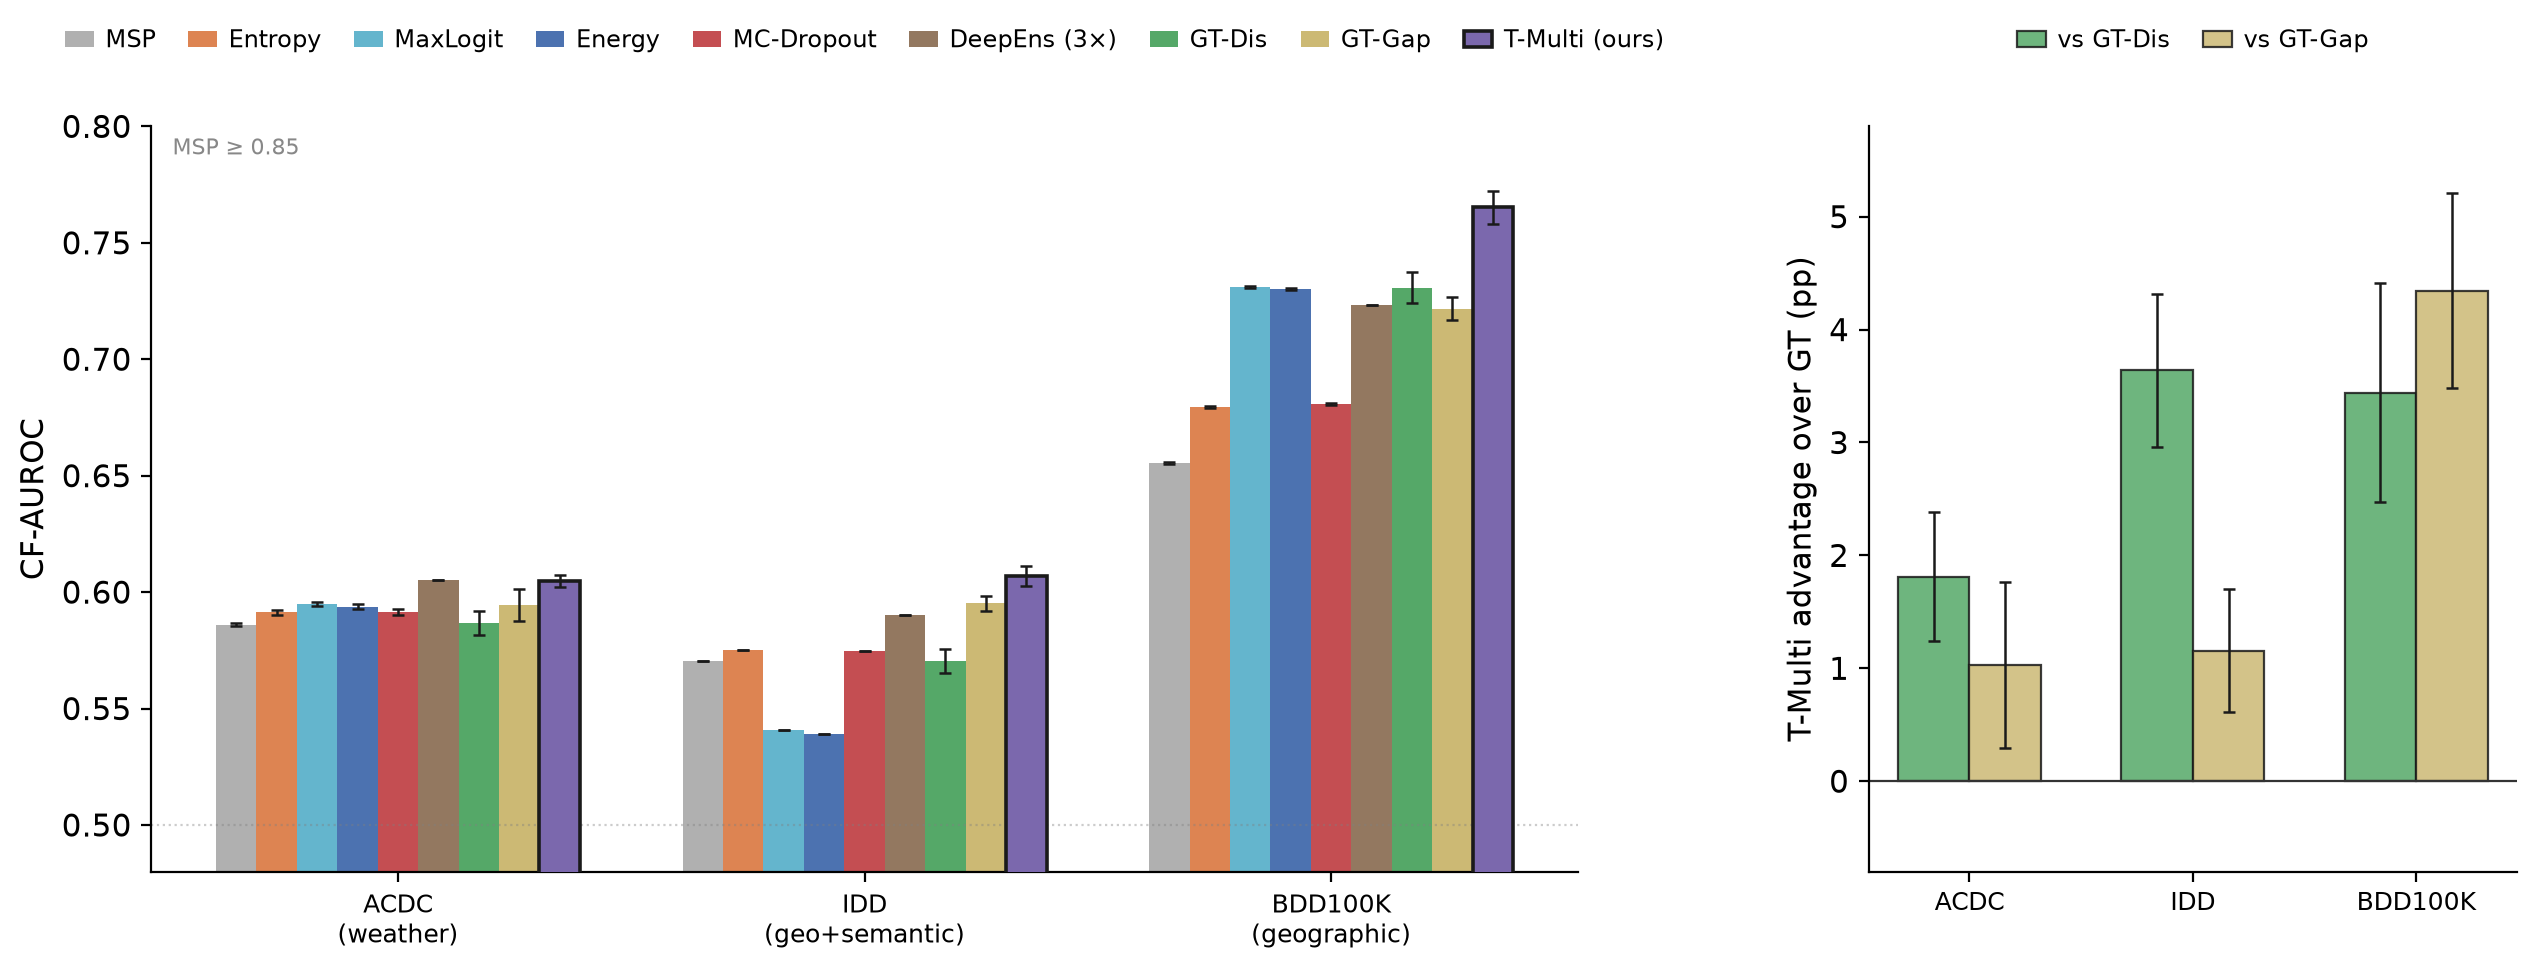
\includegraphics[width=\linewidth]{fig_teacher_vs_gt.png}
\caption{Left: CF-AUROC @ MSP$\,{\geq}\,$0.85 across methods and datasets (mit-b1). Right: T-Multi improvement over each GT baseline in percentage points.}
\label{fig:main}
\end{figure}


\paragraph{Significance.} T-Multi is competitive with the stronger uncertainty baselines, exceeding the magnitude-based scores on all three datasets and leading the $3\times$ cost Deep Ensemble on BDD (.758 vs.\ .732) and IDD (.603 vs.\ .590) while matching on ACDC (.604 vs.\ .605) at a single forward pass. Against the stricter comparator (the better of the two GT heads), T-Multi wins on all six seeds$\times$dataset cells over \{IDD, BDD\} (pooled $\Delta{=}{+}0.022$, sign-test $p\,{\approx}\,0.03$) and is small but consistent on ACDC ($+0.009$, $3/3$). A paired image bootstrap (N=$3000$ resamples with replacement within each dataset on fixed seed checkpoints) localizes to where the advantage is significant: T-Multi vs.\ GT-Dis is significant on BDD ($\Delta{=}{+}0.021$, $p{=}0.007$) and IDD ($\Delta{=}{+}0.030$, $p{<}0.001$) but not on ACDC ($\Delta{=}{+}0.014$, $p{=}0.23$). These results are consistent with the within-condition analysis (\S\ref{sec:within-condition}) to show the ACDC gain comes primarily from condition-level separation rather than within-condition ranking. The pooled advantage over GT-Dis is $+0.022$ ($p{=}0.010$) and over GT-Gap $+0.020$ ($p{=}0.040$). The image bootstrap fixes the checkpoints and quantifies sampling uncertainty over images rather than seed-uncertainty. The sign test provides across-seed evidence. With three seeds, we treat the standard-threshold gaps ($+0.6$ to $+2.0$\,pp) as suggestive rather than established, and rely on larger strict-threshold gaps (Table~\ref{tab:strict}) for the main claim.


\paragraph{Why teacher supervision transfers better.} Ground-truth labels define ``correctness'' relative to the source domain's labels. Under domain shift, the distribution of student errors changes, so the student makes different kinds of mistakes on fog vs.\ rain vs.\ geographic shift. The GT labels, by contrast, are frozen to source-domain patterns. The teacher is re-evaluated on each training image (including corrupted variants), offering an error signal that adapts to the input. Under domain shift, teacher-derived dense targets transfer better than dense targets defined only by source-domain correctness.


\begin{table}[H]
\centering
\small
\setlength{\tabcolsep}{5pt}
\caption{Student vs.\ teacher reference quality by dataset (mit-b1). mIoU is the macro average over classes. S--T disagree is the mean per-image fraction of pixels where $\hat y^S\!\neq\!\hat y^T$; the last column is the mean per-image fraction of pixels where the student is confidently wrong but the teacher is correct---the recoverable silent failures the teacher target exposes.}
\label{tab:diag}
\begin{tabular}{lcccc}
\toprule
 & Student mIoU & Teacher mIoU & S--T disagree & Conf.-wrong, T-right \\
\midrule
Cityscapes (in-dom.) & .691 & .774 & 4.2\% & 0.6\% \\
ACDC & .405 & .517 & 16.6\% & 4.1\% \\
IDD & .459 & .532 & 8.7\% & 1.5\% \\
BDD & .445 & .554 & 10.6\% & 3.0\% \\
\bottomrule
\end{tabular}
\end{table}

Table~\ref{tab:diag} shows the teacher is a stronger reference on each dataset (mIoU gap $+0.07$ to $+0.11$), and the student--teacher disagreement and the fraction of pixels where the student is confidently wrong but the teacher is correct grow from $0.6\%$ of pixels in-domain to $3$--$4\%$ on ACDC and BDD. Binary ground-truth targets $d^{\mathrm{GT}}$ consider all student pixel errors equally, including shared failures with the teacher. The continuous GT target $r^{\mathrm{GT}}$ is the student's cross-entropy and varies with student confidence. The teacher excess-loss target $r^{T}$ measures the model residual against the teacher's preferred class, subtracting the teacher's own loss. Thus, it tends to decrease shared failures, where the student and teacher are similarly confident and incorrect on the same class, and is only large when the student performs worse than the teacher. Because recoverable confident failures become denser and more decisive under shift (Table~\ref{tab:diag}), this is consistent with the teacher's advantage being largest under shift at strict confidence (Table~\ref{tab:strict}). This carries a risk, as the teacher is a weaker reference than the student on $12$--$21\%$ of images per dataset (by more than $5$\,pp mIoU on $2.5$--$7.4\%$), where the teacher target may flag a locally correct student prediction as risky. A per-pixel correctness breakdown shows the recoverable case is much more common than the harmful case. On ACDC (resp.\ BDD), pixels where the student is wrong but the teacher is correct account for $9.4\%$ ($6.7\%$) of all valid pixels, compared to only $2.4\%$ ($2.1\%$) where the student is correct and the teacher is wrong. When considering high-confidence pixels (MSP$\,{\geq}\,0.9$), the recoverable fraction still exceeds the harmful case with $5.3\%$ vs.\ $1.3\%$ on ACDC and $3.8\%$ vs.\ $1.0\%$ on BDD. The teacher's net mIoU advantage ($+0.06$ to $+0.09$) therefore wins, and T-Multi still beats the GT heads (Table~\ref{tab:main}).

\subsection{High-confidence failure detection}


\begin{table}[H]
\centering
\small
\setlength{\tabcolsep}{4pt}
\caption{CF-AUROC at strict MSP thresholds (mit-b1). At MSP$\,{\geq}\,$0.95, probability-based post-hoc scores converge towards random, compared to magnitude-based scores (MaxLogit, energy) which are more resilient. T-Multi maintains discrimination, with a growing advantage over GT. $n$ is the number of confident images at each threshold. ACDC at MSP $\geq 0.97$ has $n=23$, so results have been omitted.}
\label{tab:strict}
 \begin{tabular}{llrccccccc}
\toprule
 & $\tau$ & $n$ & MSP & MaxL & Energy & MC-D & GT-Dis & GT-Gap & \textbf{T-Multi} \\
\midrule
\multirow{2}{*}{ACDC}
 & 0.85 & 397 & \loss{.587} & .596 & .594 & .593 & .589 & .599 & \win{.604} \\
 & 0.95 & 144 & .437 & .534 & .534 & \loss{.432} & .501 & .508 & \win{.563} \\
\midrule
\multirow{3}{*}{IDD}
 & 0.85 & 976 & .573 & \loss{.543} & .539 & .577 & .575 & .592 & \win{.603} \\
 & 0.95 & 634 & \loss{.501} & .505 & .505 & .509 & .506 & .519 & \win{.541} \\
 & 0.97 & 231 & \loss{.485} & .557 & \win{.564} & .499 & .492 & .513 & .502 \\
\midrule
\multirow{3}{*}{BDD}
 & 0.85 & 987 & \loss{.657} & .732 & .730 & .682 & .738 & .716 & \win{.758} \\
 & 0.95 & 622 & \loss{.487} & .589 & .592 & .530 & .608 & .573 & \win{.662} \\
 & 0.97 & 169 & \loss{.341} & .380 & .380 & .396 & .439 & .431 & \win{.566} \\
\bottomrule
\end{tabular}
\end{table}


The T-Multi advantage over GT grows at stricter thresholds. At MSP$\,{\geq}\,$0.95 on ACDC, T-Multi 0.563 vs.\ GT-Gap 0.508 (+5.5\,pp). On BDD at 0.95, T-Multi 0.662 vs.\ GT-Dis 0.608 (+5.4\,pp). At 0.97 on BDD, T-Multi maintains 0.566 while GT-Dis drops to 0.439 (+12.7\,pp). The widening gap suggests the teacher signal provides more robust features in the hardest cases. On ACDC and BDD, MaxLogit and Energy's AUROC declines steeply with tighter MSP thresholds as softmax saturation compresses the confident subset's logit-magnitude spread, whereas on IDD they stay the best at MSP$\,{\geq}\,$0.97 (0.557/0.564).


\begin{figure}[H]
\centering
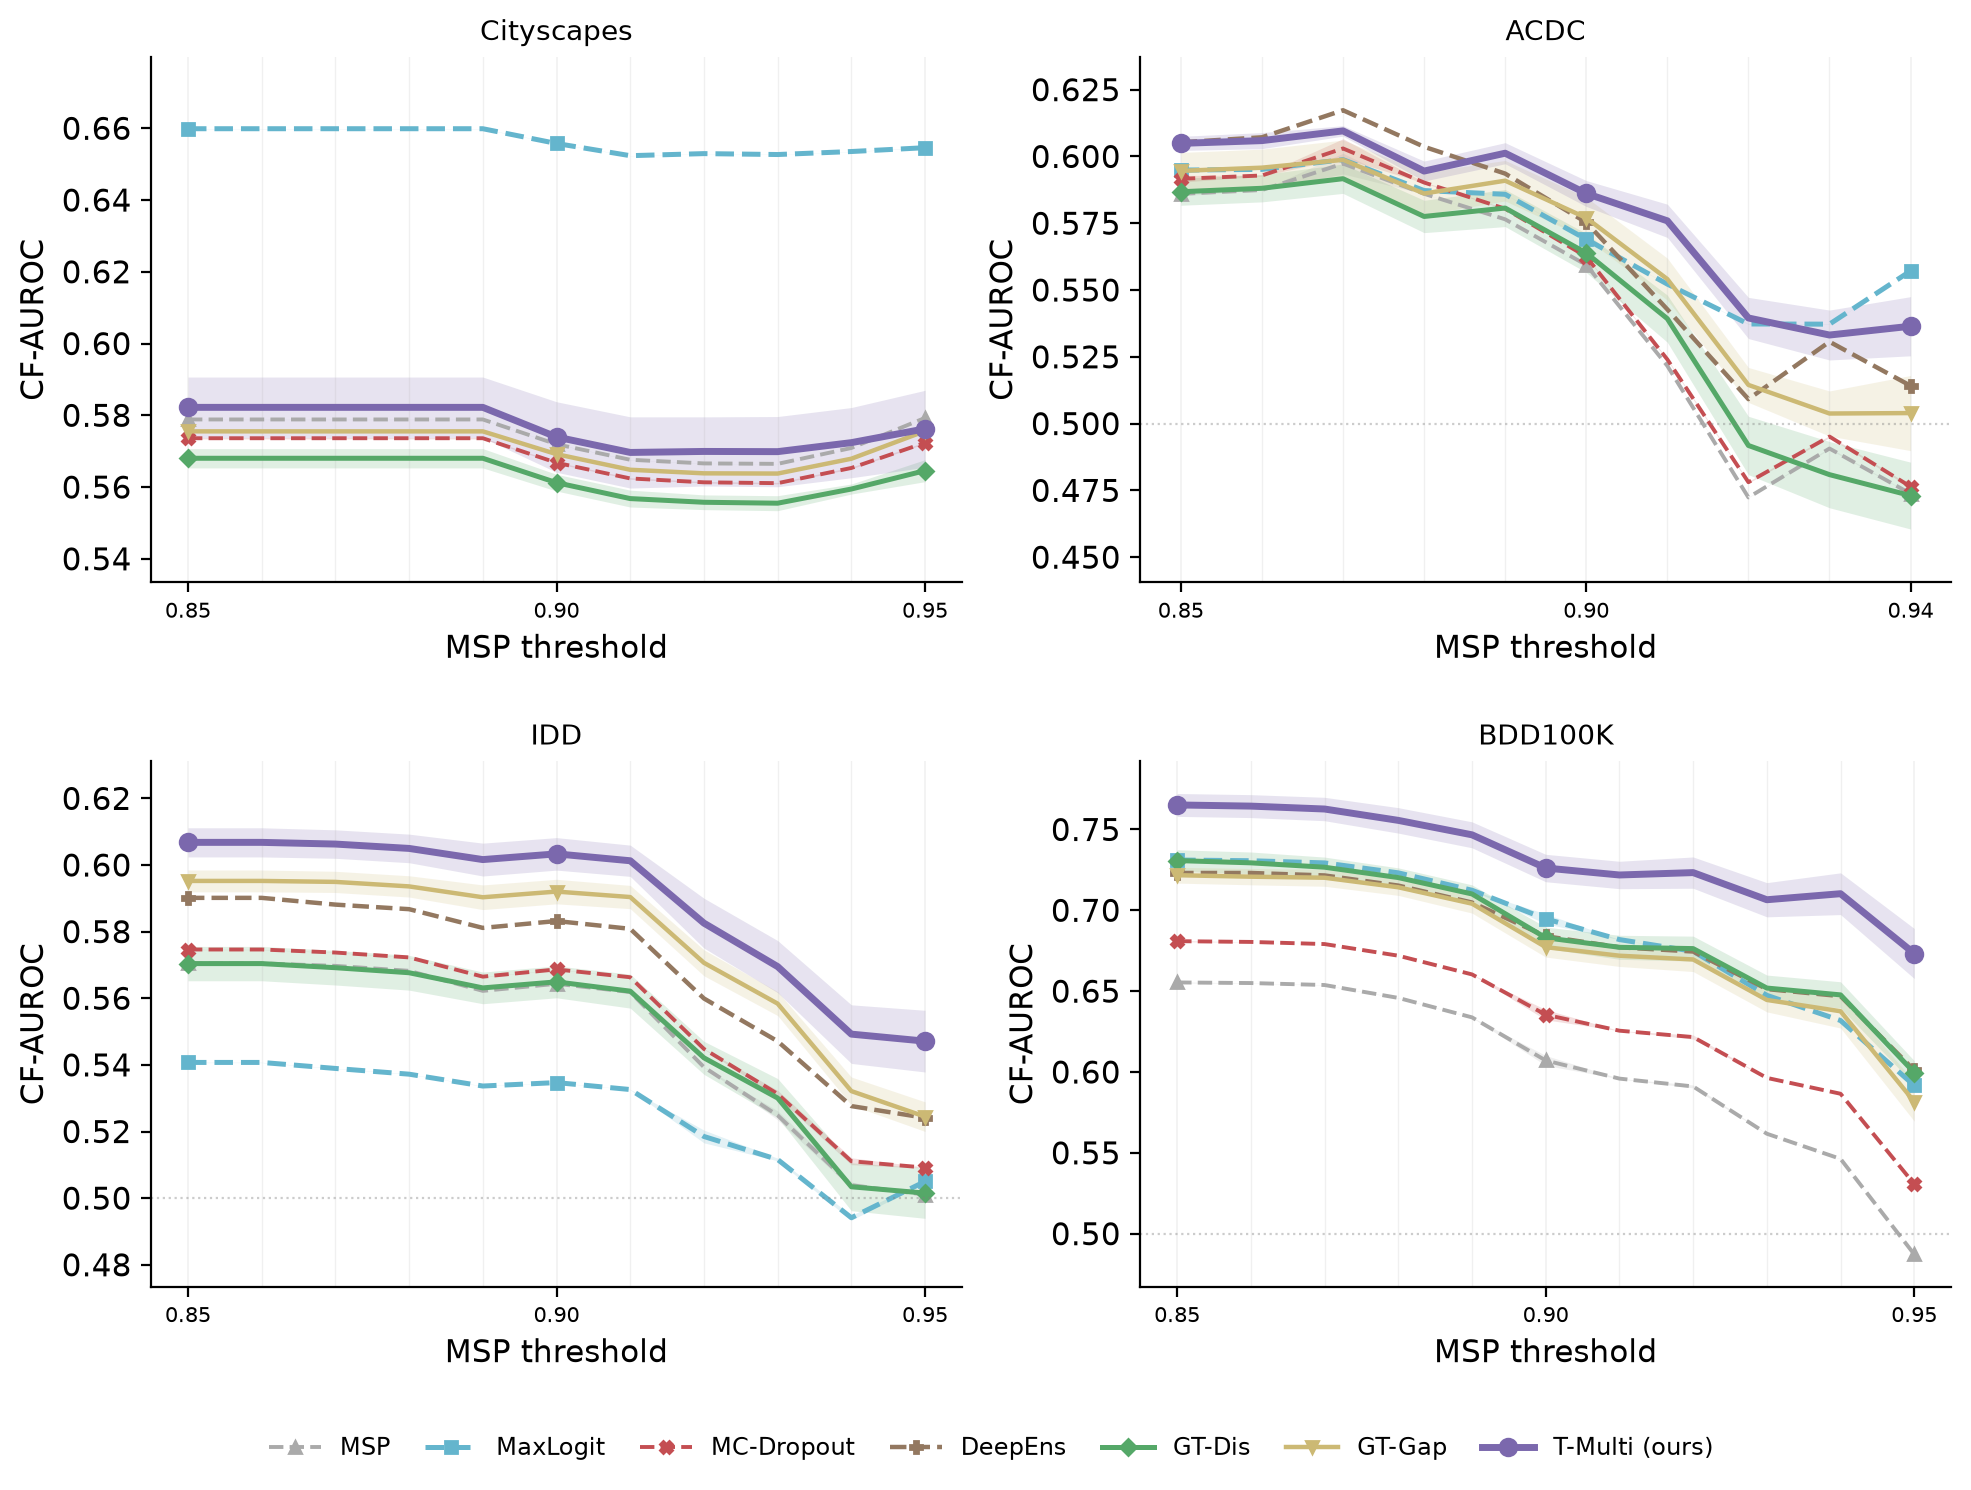
\includegraphics[width=\linewidth]{fig_threshold_sweep.png}
\caption{CF-AUROC across MSP thresholds (mit-b1). T-Multi degrades most slowly on ACDC and BDD.}
\label{fig:sweep}
\end{figure}


\subsection{Within-condition analysis} \label{sec:within-condition}






\begin{table}[H]
\centering
\small
\setlength{\tabcolsep}{4pt}
\caption{Within-condition failure AUROC (ACDC, mit-b1). Bottom rows: macro-average (mean of per-condition AUROCs), condition-only baseline (assign each image its condition's mean risk), and pooled. The gap between pooled and macro-averaged results shows that much of the pooled gain comes from separating conditions rather than from uniformly stronger failure rankings within each condition.}
\label{tab:within}
\begin{tabular}{lcccccc}
\toprule
Cond. & MSP & MaxL & MC-D & GT-Dis & GT-Gap & \textbf{T-Multi} \\
\midrule
Fog & .495 & .576 & .503 & .519 & .521 & \win{.600} \\
Night & .607 & \win{.760} & .625 & .670 & .659 & .590 \\
Rain& .734 & .628 & .749 & .747 & .762 & \win{.764} \\
Snow& .552 & \win{.664} & .554 & .602 & .628 & .636 \\
\midrule
Macro-avg & .597 & \win{.657} & .608 & .634 & .643 & .648 \\
\midrule
Condition-only & \multicolumn{6}{c}{0.816 (assigns condition mean risk)} \\
Pooled& .692 & .927 & .710 & .910 & .903 & \win{.928} \\
\bottomrule
\end{tabular}
\end{table}


\paragraph{Condition-only baseline.} A score that assigns each image its condition's mean student risk achieves 0.816 pooled F-AUROC. T-Multi's pooled 0.928 exceeds this by +11.2\,pp, demonstrating it identifies signal beyond the condition class.


\paragraph{Macro-average.} Averaging across conditions removes the between-condition signal entirely. MaxLogit leads (0.657), followed by T-Multi (0.648) and GT-Gap (0.643). T-Multi beats MSP (+5.1\,pp) and MC-Dropout (+4.0\,pp) within-condition, but MaxLogit's within-condition ranking is stronger by 0.9\,pp. T-Multi's pooled advantage over MaxLogit thus comes mainly from the condition-level signal rather than learned patterns.


\paragraph{Night weakness.} Night images have uniformly high student risk (mean 0.82, std 0.05; nearly all are failures), leaving almost no within-condition variance to detect. The guardrail score is near-constant within night (std = 0.07, corr = 0.25 with student risk), while MaxLogit's logit magnitudes vary more (std = 0.58, $|$corr$|$ = 0.43).


\begin{figure}[H]
\centering
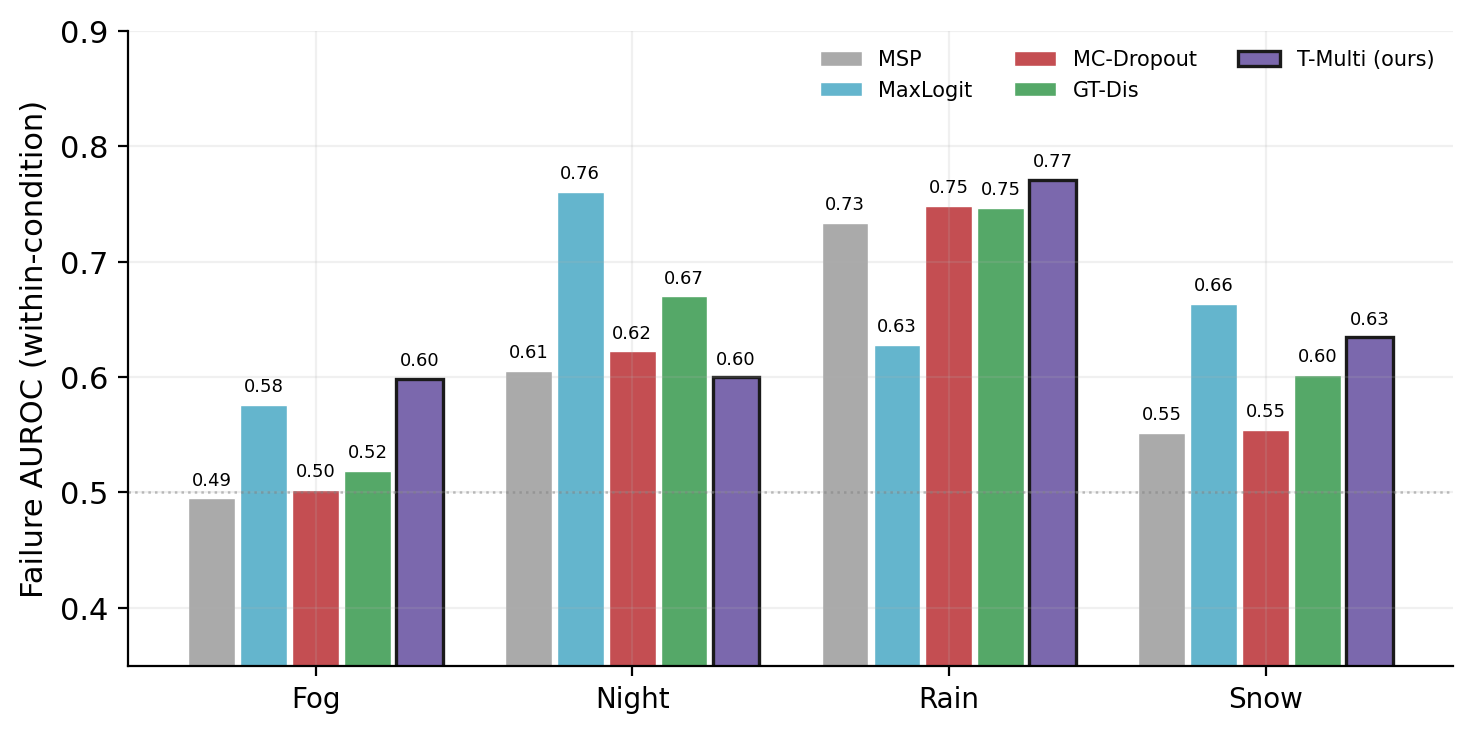
\includegraphics[width=0.9\linewidth]{fig_within_condition.png}
\caption{Within-condition failure AUROC on ACDC (mit-b1). T-Multi wins fog and rain; MaxLogit dominates night and snow.}
\label{fig:within}
\end{figure}


\subsection{Supervision mode ablation}


\begin{table}[H]
\centering
\small
\setlength{\tabcolsep}{4pt}
\caption{Full ablation of supervision modes (b1, CF-AUROC @ MSP$\,{\geq}\,$0.85). Teacher-supervised modes are strongest on BDD, while ACDC remains mixed across target types.}
\label{tab:ablation}
\begin{tabular}{lcccccccc}
\toprule
 & MSP & Scalar & GT-Dis & GT-Gap & T-Dis & T-Gap & T-Multi \\
\midrule
City & .579 & .613 & .566 & .576 & .574 & .583 & .571 \\
ACDC & .587 & .569 & .589 & .599 & .582 & .597 & \win{.604} \\
IDD & .573 & .570 & .575 & .592 & .585 & .617 & .603 \\
BDD & .657 & .754 & .738 & .716 & .745 & .747 & \win{.758} \\
\bottomrule
\end{tabular}
\end{table}


The ablation separates the two design axes for the guardrail head: the supervision source (teacher vs.\ GT) and the target shape (dense disagreement, dense gap, or both). Along the source axis, the teacher signal's largest benefit is on BDD, where every teacher mode beats every GT variant (best teacher 0.758 vs.\ best GT 0.738, $+2.0$\,pp); it narrows on IDD ($+2.5$\,pp for T-Gap over GT-Gap) and is marginal on ACDC ($+0.5$\,pp for T-Multi), consistent with the per-condition analysis that shows the ACDC gains are primarily from learned condition rather than within-condition rankings. Along the shape axis, a continuous gap target consistently outperforms binary disagreement: T-Dis is inferior to T-Gap and T-Multi on every OOD dataset and even loses to both GT variants on ACDC ($0.582$ vs.\ $0.589$/$0.599$). T-Multi combines both axes and is the default.


\paragraph{Scalar baseline as negative control.} The scalar row trains the same architecture on a single image-level target ($\text{student\_risk}\!-\!\text{teacher\_risk}$) instead of dense per-pixel supervision. Under the joint evaluation, results degrade to near-MSP performance on ACDC ($0.569$) and IDD ($0.570$), confirming that per-pixel supervision makes the teacher signal usable as a score. The image-level benefit target itself is structurally unlearnable (cross-validated $R^2 \leq 0.06$). Its BDD result ($0.754$) comes from student-risk features the head picks up incidentally rather than from predicting its stated target. By contrast, the dense teacher-supervised modes retain a stronger signal in the high-confidence regime (Table~\ref{tab:strict}).


\begin{figure}[H]
 \centering
 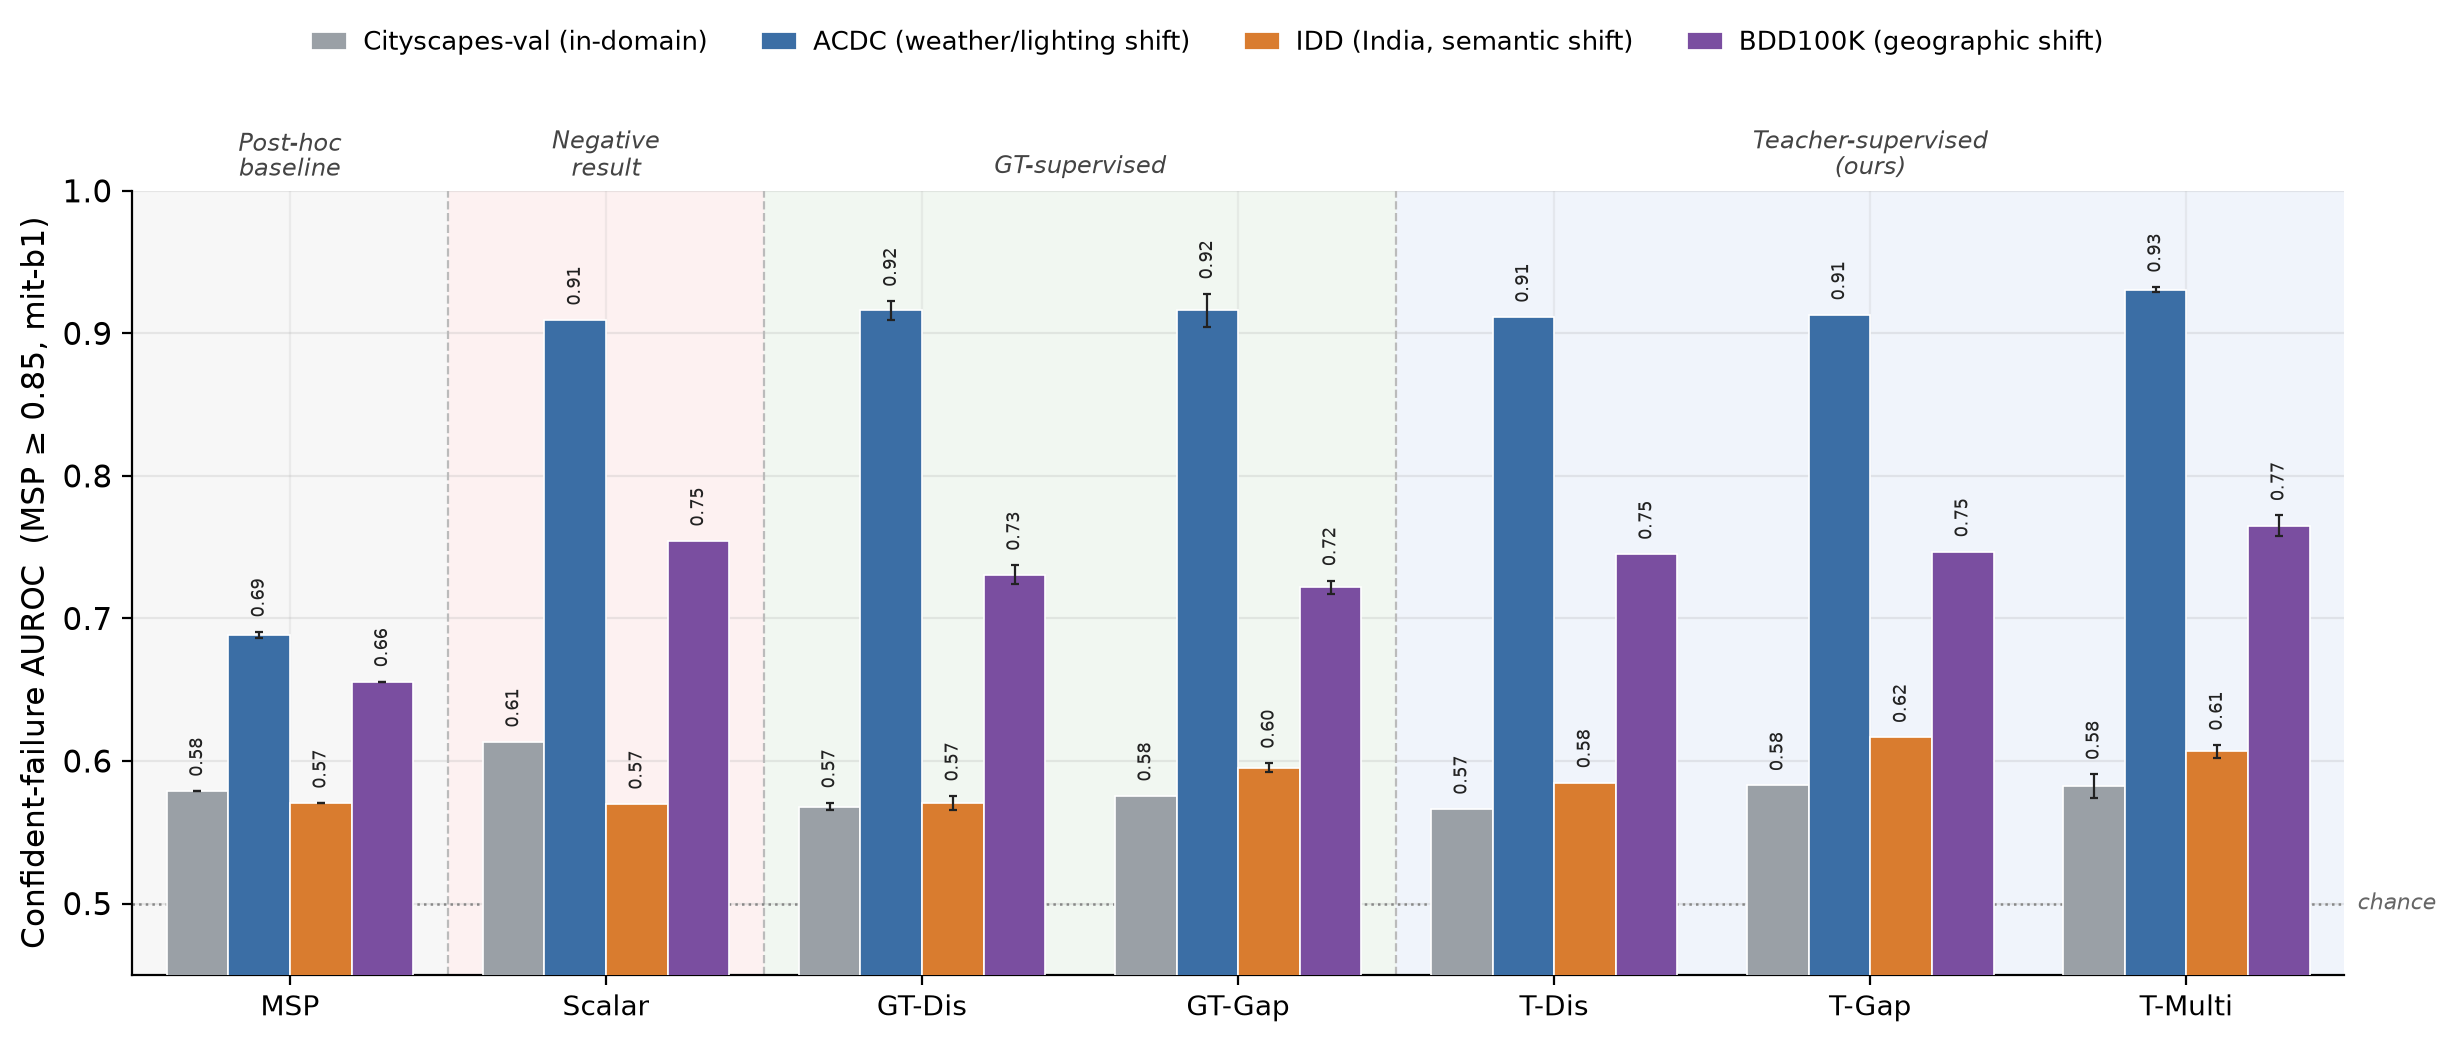
\includegraphics[width=\linewidth]{fig_supervision_ablation.png}
\caption{Full supervision ablation (mit-b1, CF-AUROC @ MSP$\,{\geq}\,$0.85). Teacher-supervised modes are strongest on BDD and mixed on ACDC; T-Multi is the best overall teacher-supervised variant.}
 \label{fig:ablation}
\end{figure}


\subsection{Confidence features close the gap to post-hoc scores}
\label{sec:conffeat}


The teacher head is competitive with, but does not uniformly beat, magnitude-based post-hoc scores such as energy and MaxLogit (Tables~\ref{tab:main},~\ref{tab:strict}). Because a shallow head does not easily recover these magnitude statistics from the raw logits, we evaluate the confidence variant (\S\ref{sec:conffeat-method}) which feeds the per-pixel energy and max-logit directly into the head as additional input channels, so the single learned score fuses both. We train it only with the frozen student / teacher on the same three SegFormer backbones.


\begin{table}[H]
\centering
\small
\setlength{\tabcolsep}{6pt}
\caption{Confidence-feature head vs.\ the energy score (CF-AUROC @ MSP$\,{\geq}\,$0.85 on ACDC). Pooled is over all $3{\times}5{=}15$ runs. Feeding energy/max-logit into the head as input channels outperforms the energy score alone across five seeds.}
\label{tab:conffeat}
\begin{tabular}{lcccc}
\toprule
Method & b0 & b1 & b2 & Pooled \\
\midrule
Energy score      & .590 & .595 & .582 & .589\,{\scriptsize$\pm$.005} \\
Guardrail $+$ conf.\ features (ours) & \win{.624} & \win{.620} & \win{.589} & \win{.611\,{\scriptsize$\pm$.017}} \\
\midrule
$\Delta$ vs.\ energy & \win{+3.4} & \win{+2.5} & \win{+0.7} & \win{+2.2} \\
\bottomrule
\end{tabular}
\end{table}


Table~\ref{tab:conffeat} shows the confidence-feature head beats energy by $+2.2$\,pp pooled (14/15 runs; paired sign-test $p{=}0.001$, $t{=}6.3$). This shows the teacher head wins over energy. The identical head trained with and without the two confidence channels isolates the effect of the architecture from the score: the channels lift CF-AUROC by $+1.9$\,pp ($5/6$ runs), independent of the teacher-vs-GT axis. The gain is specific to domain shift, wherein in-domain (Cityscapes), the energy score is stronger (e.g., b1 $.659$ vs $.612$), so the learned score is useful where post-hoc magnitude scores are least reliable. Merging the head's output with the energy score at inference gives no additional gain over the confidence-feature head in this metric, so we report the single learned score.


\subsection{Inference cost and reliability comparison}
\label{sec:latency}


Failure detection is only practical when the inference cost is justified by the reliability gain. Table~\ref{tab:latency-auroc} reports per-image inference cost alongside CF-AUROC at MSP$\,\geq\,$0.95, the high-confidence regime where post-hoc scores are weakest and silent failures are most dangerous.


\begin{table}[htpb]
 \centering
 \small
 \setlength{\tabcolsep}{6pt}
 \caption{Per-image inference latency vs.\ confident-failure AUROC at MSP$\,\geq 0.95$ on three datasets (mit-b1, 1$\times$NVIDIA L40S, batch size=4). ACDC is the per-condition mean over fog/night/rain/snow. Latencies are reported as the median over 500 Cityscapes-val images after 50 warm-up passes, with CUDA synchronization on each forward pass. The teacher is an upper bound, where routing every image to the teacher resolves confident failures at full teacher latency.}
 \label{tab:latency-auroc}
 \begin{tabular}{lccccc}
  \toprule
  Method & Latency (ms) & ACDC & IDD & BDD100K & Mean OOD \\
  \midrule
  Student (MSP)        & 4.9 & .437 & .501 & .487 & .475 \\
  MaxLogit           & 4.9 & .534 & .505 & .589 & .543 \\
  MC-Dropout (4 passes)    & 25.2 & .432 & .509 & .530 & .490 \\
  Student + guardrail (T-Multi, ours) & 16.8 & .563 & .541 & .662 & .589 \\
  Teacher (full inference)  & 26.1 & 1.00 & 1.00 & 1.00 & 1.000 \\
  \bottomrule
 \end{tabular}
\end{table}


\paragraph{Pareto analysis.} The guardrail improves over MC-Dropout, with $+9.9$\,pp higher mean AUROC at $33\%$ lower latency despite MC-Dropout requiring four stochastic forward passes. Against MaxLogit, the tradeoff is $+11.9$\,ms of latency for $+4.6$\,pp mean AUROC, widening to $+7.3$\,pp on BDD100K. Against the teacher upper bound, the guardrail closes $22\%$ of the MSP-to-teacher gap on average ($34\%$ on BDD) without ever invoking the teacher.


\paragraph{Cost decomposition.} The guardrail head adds $11.9$\,ms to the student's $4.9$\,ms forward pass, for a total of $16.8$\,ms. This overhead is independent of backbone size, as the head uses the segmentation output resolution. We report measured latency for b1 only. MC-Dropout's $25.2$\,ms uses four stochastic student passes, and the teacher's $26.1$\,ms is a single $84.7$M-parameter forward pass. The guardrail offers a fixed cost while beating both alternatives in latency. A Deep Ensemble is a comparative point on this axis as it does not exceed the single-pass guardrail on failure detection under shift (Table~\ref{tab:main}) and yields a higher selective risk (AURC $.628$ vs.\ $.610$ on ACDC-b1, Fig.~\ref{fig:deepens-rc}). With three independent students, it is dominated by the cost-reliability trade-off.


\begin{figure}[H]
 \centering
 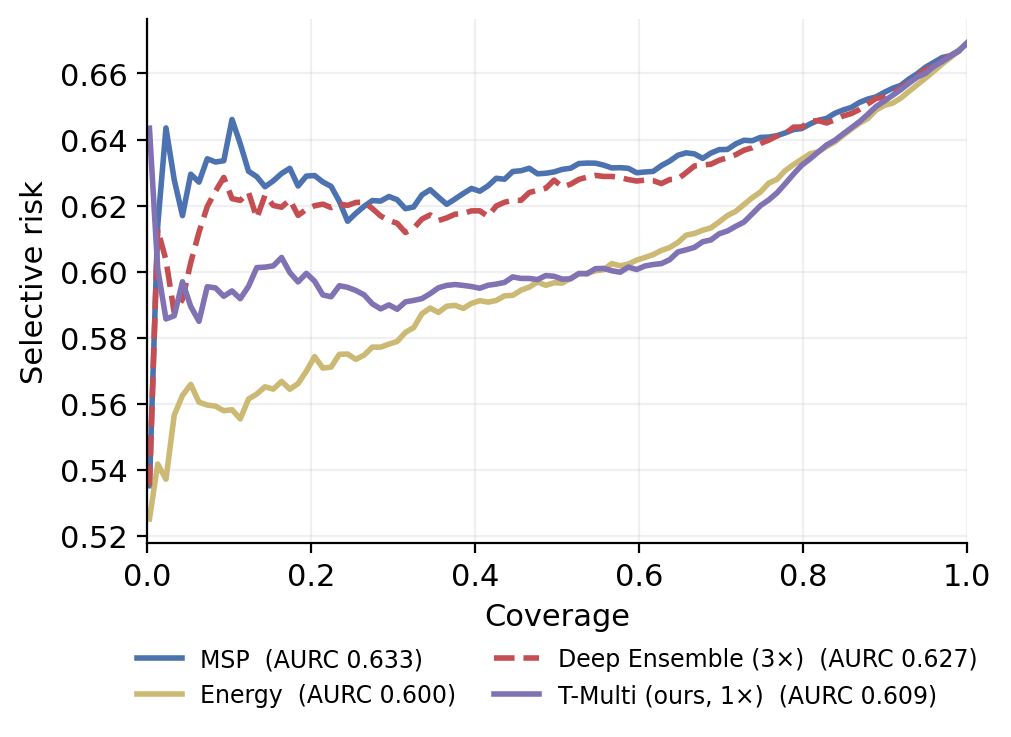
\includegraphics[width=0.62\linewidth]{fig_deep_ensemble.png}
 \caption{Risk-coverage on ACDC (mit-b1). The single-pass guardrail (T-Multi) has a lower selective risk at each coverage than the $3\times$-cost Deep Ensemble. The post-hoc energy score is comparably strong.}
 \label{fig:deepens-rc}
\end{figure}


\paragraph{Selective deferral.} The guardrail's risk score gates teacher invocation. If the teacher is invoked on flagged inputs at flag rate $f$, the expected per-frame latency is
\[
\mathbb{E}[L] = L_{\text{student}} + L_{\text{guardrail}} + f \cdot L_{\text{teacher}}.
\]
At $f = 0.1$, $\mathbb{E}[L] = 19.4$\,ms: $15\%$ above guardrail-alone latency and $26\%$ below full teacher inference. Table~\ref{tab:defer} shows mIoU benefit recovered, where routing the $10\%$ highest-risk frames to the teacher recovers $12.8\%$ of the total student$\to$teacher mIoU benefit at $19.4$\,ms, competitive with the best post-hoc gate and well above random deferral ($9.9\%$). At these low budgets, the recovered benefit is similar across all detectors, because the deferral acts on the same easily ranked failures. The guardrail's distinct advantage is in high-confidence detection (Table~\ref{tab:strict}) rather than in low-budget deferral mIoU.

\begin{table}[H]
\centering
\small
\setlength{\tabcolsep}{6pt}
\caption{Teacher-deferral benefit vs.\ cost (mit-b1, pooled over ACDC/IDD/BDD). Each detector routes its highest-risk fraction $f$ of frames to the teacher. Entries are the percentage of the total student$\to$teacher mIoU benefit recovered. $\mathbb{E}[L]$ is the per-frame latency (\,$16.8 + f\,{\cdot}\,26.1$\,ms\,). Best non-oracle detector per row in bold.}
\label{tab:defer}
\begin{tabular}{lcccccc}
\toprule
$f$ & $\mathbb{E}[L]$ (ms) & Random & MSP & MaxL & \textbf{T-Multi} & Oracle \\
\midrule
0.05 & 18.1 & 5.2 & 5.7 & \win{6.5} & 6.2 & 15.7 \\
0.10 & 19.4 & 9.9 & 12.6 & 12.7 & \win{12.8} & 27.9 \\
0.20 & 22.0 & 19.0 & 24.0 & \win{24.7} & 24.4 & 47.2 \\
\bottomrule
\end{tabular}
\end{table}


\section{Discussion}


Our results support two main conclusions. First, learned dense failure predictors are competitive with standard post-hoc confidence metrics under distribution shift. Second, within this class of methods, teacher-guided supervision generally outperforms matched GT supervision under shift. This gain is minor at typical operation, but increases in the high-confidence regime, where silent failures are most dangerous. Additionally, the comparison to post-hoc baselines is not uniform: MaxLogit is a strong baseline, especially for structured weather shift, whereas the teacher-guided head degrades more gracefully on ACDC and BDD as confidence thresholds tighten. Together, these results suggest that the proposed method is most useful when failures are not well captured by a single global confidence metric and require learned spatial structure. Additionally, although a magnitude score such as energy or MaxLogit adds no information beyond the student logits, feeding it into the head as an input channel recovers a single learned score that surpasses either score individually under shift.


The ablations show that most of the improvement over MSP comes from learning a dense predictor on top of frozen student logits with corruption-aware training. Teacher supervision also provides a smaller but consistent benefit over GT supervision under shift. This also helps position the method relative to ConfidNet-style approaches \cite{corbiere2019confidnet}: our GT-Dis baseline is the matched GT-supervised analog, so the teacher-versus-GT comparison isolates the value of the teacher signal rather than changes in architecture or optimization. Overall, teacher supervision improves transfer once a strong, dense failure-prediction architecture is in place.


The method also has limitations. The within-condition analysis shows that the method is not uniformly superior: night scenes are difficult, and in-domain performance has little to no advantage over confidence baselines. The confidence-feature gain also decreases monotonically with student capacity (b0 $+3.4$, b1 $+2.5$, b2 $+0.7$\,pp), which suggests it helps most for the smallest, most heavily compressed students and adds little once the student is large (b2). In addition, the method does not benefit from teacher inference at test time, although the risk can trigger teacher deferral. The conclusion, supported by the results, is that teacher-guided dense supervision improves failure detection under domain shift, with the clearest benefit in the high-confidence regime, where post-hoc confidence is least reliable.






\paragraph{Broader impacts.}
This work estimates risk for semantic segmentation under domain shift, with a potential positive impact in safety-critical perception settings (such as driving) by detecting high-confidence failures before downstream decisions are made using them. However, the guardrail is not a safety certificate: false negatives could still allow unsafe predictions, and false positives may unnecessarily defer and degrade system performance. The experiments use driving-scene datasets, so deployment could also learn dataset biases across geography, weather, lighting, and road infrastructure. Any real-world use should treat the guardrail as a component of a larger safety stack rather than a standalone guarantee of safety.


\section{Related work}


\paragraph{Selective prediction.} Selective prediction abstains on low-confidence inputs, exchanging decreased coverage for lower risk~\cite{geifman2017selective}. Standard post-hoc scores include MSP~\cite{hendrycks2017baseline}, temperature scaling~\cite{guo2017calibration}, MC-Dropout~\cite{gal2016dropout} and MaxLogit~\cite{hendrycks2022scaling}. Classical alternatives are Deep Ensembles~\cite{lakshminarayanan2017deepensembles}, where predictive uncertainty degrades gracefully under distribution shift ~\cite{ovadia2019trust}, and aleatoric/epistemic uncertainty for dense vision~\cite{kendall2017uncertainties}. Learned confidence heads move beyond these scores. are standard post-hoc scores. SelectiveNet dually trains a predictor and a reject option~\cite{geifman2019selectivenet}, and ConfidNet trains an auxiliary head to predict the True Class Probability from ground-truth labels~\cite{corbiere2019confidnet}. Recent work standardizes measurements for failure detection and warns that it is easily mis-evaluated~\cite{jaeger2023call, traub2024overcoming}. We report AURC and confident-failure AUROC to ensure a rigerous assessment of reliability. Our method retains the learned-head, but replaces ground-truth-derived dense targets with teacher-derived dense targets, which transfer better under shift because they adapt to the teacher's response.

\paragraph{Out-of-distribution and anomaly segmentation.} For dense prediction, reliability is often considered a per-pixel OOD/anomaly detection. Standardized max-logit for road obstacles~\cite{jung2021standardized}, entropy maximization with meta-classification~\cite{chan2021entropy}, resynthesis/reconstruction discrepancy~\cite{dibiase2021pixel}, and predicting a segmentation network's own errors from local adversarial perturbations~\cite{besnier2021triggering}. Deterministic single-pass uncertainty~\cite{mukhoti2023deep}, evidential mask transformers ~\cite{schmidt2025prior2former}, andgeneralize-or-detect training under multiple shifts~\cite{gao2024generalize} consider the same goal. These methods use a single standalone model; whereas we instead ask whether a teacher used to distill a compressed student also finds a better supervision signal for the student's image-level failure detection under shift.

\paragraph{Uncertainty distillation.} Deep Ensembles transfer uncertainty from ensemble teachers, typically requiring 3--5 independently trained models ~\cite{lakshminarayanan2017deepensembles}. DUDES distills ensemble uncertainty into a single-pass segmentation model ~\cite{landgraf2024dudes}. Our method is complementary and uses only a single teacher and a 67K-parameter head, rather than distilling ensemble uncertainty.


\paragraph{Knowledge distillation for segmentation.} SegFormer and related architectures are compressed via standard KD ~\cite{hinton2015distilling, xie2021segformer}. Structured KD extends this with pixel-wise, pairwise, and holistic dense-prediction objectives ~\cite{liu2019structuredkd}. Prior work focuses on closing the mIoU gap. Our work complements this by equipping the distilled student with a post-distillation reliability measure.


\section{Conclusion}


Teacher-supervised dense targets provide a stronger signal for failure detection under distribution shift than dense targets derived from ground-truth correctness. A 67K-parameter head trained with these targets outperforms identically-architected GT-supervised heads under domain shift (+0.6 to +2.0\,pp at standard thresholds, widening to +5 to +13\,pp at strict thresholds on ACDC and BDD), while in-domain behavior remains mixed. Compared to post-hoc confidence baselines, the guardrail remains competitive overall, stays close to MaxLogit on structured weather shift, and exceeds it on diffuse geographic shift (BDD, +2.6\,pp CF-AUROC). The single-pass guardrail additionally Pareto-dominates MC-Dropout, matches or beats a $3\times$-cost Deep Ensemble on failure detection under shift, and closes $22\%$ of the MSP-teacher gap on out-of-distribution data without ever invoking the teacher (\S\ref{sec:latency}). For low-budget teacher routing over the full input distribution, the guardrail's advantage is not shown as the advantage is in discrimination within the high-confidence regime rather than low-budget deferral.


The main driver of improvement over post-hoc methods is the guardrail architecture with corruption augmentation, which benefits all learned heads, including GT-supervised ones. The teacher signal adds a secondary but consistent gain. The guardrail is most useful when failure patterns vary across images (ACDC, BDD) and offers less additional benefit when that variation is limited (IDD, Cityscapes).


{\small
\bibliographystyle{unsrt}
\bibliography{refs}
}
\raggedbottom
\appendix


\section{Silent confident failure comparison}
\label{sec:qualitative-snow}


\begin{figure}[H]
 \centering
 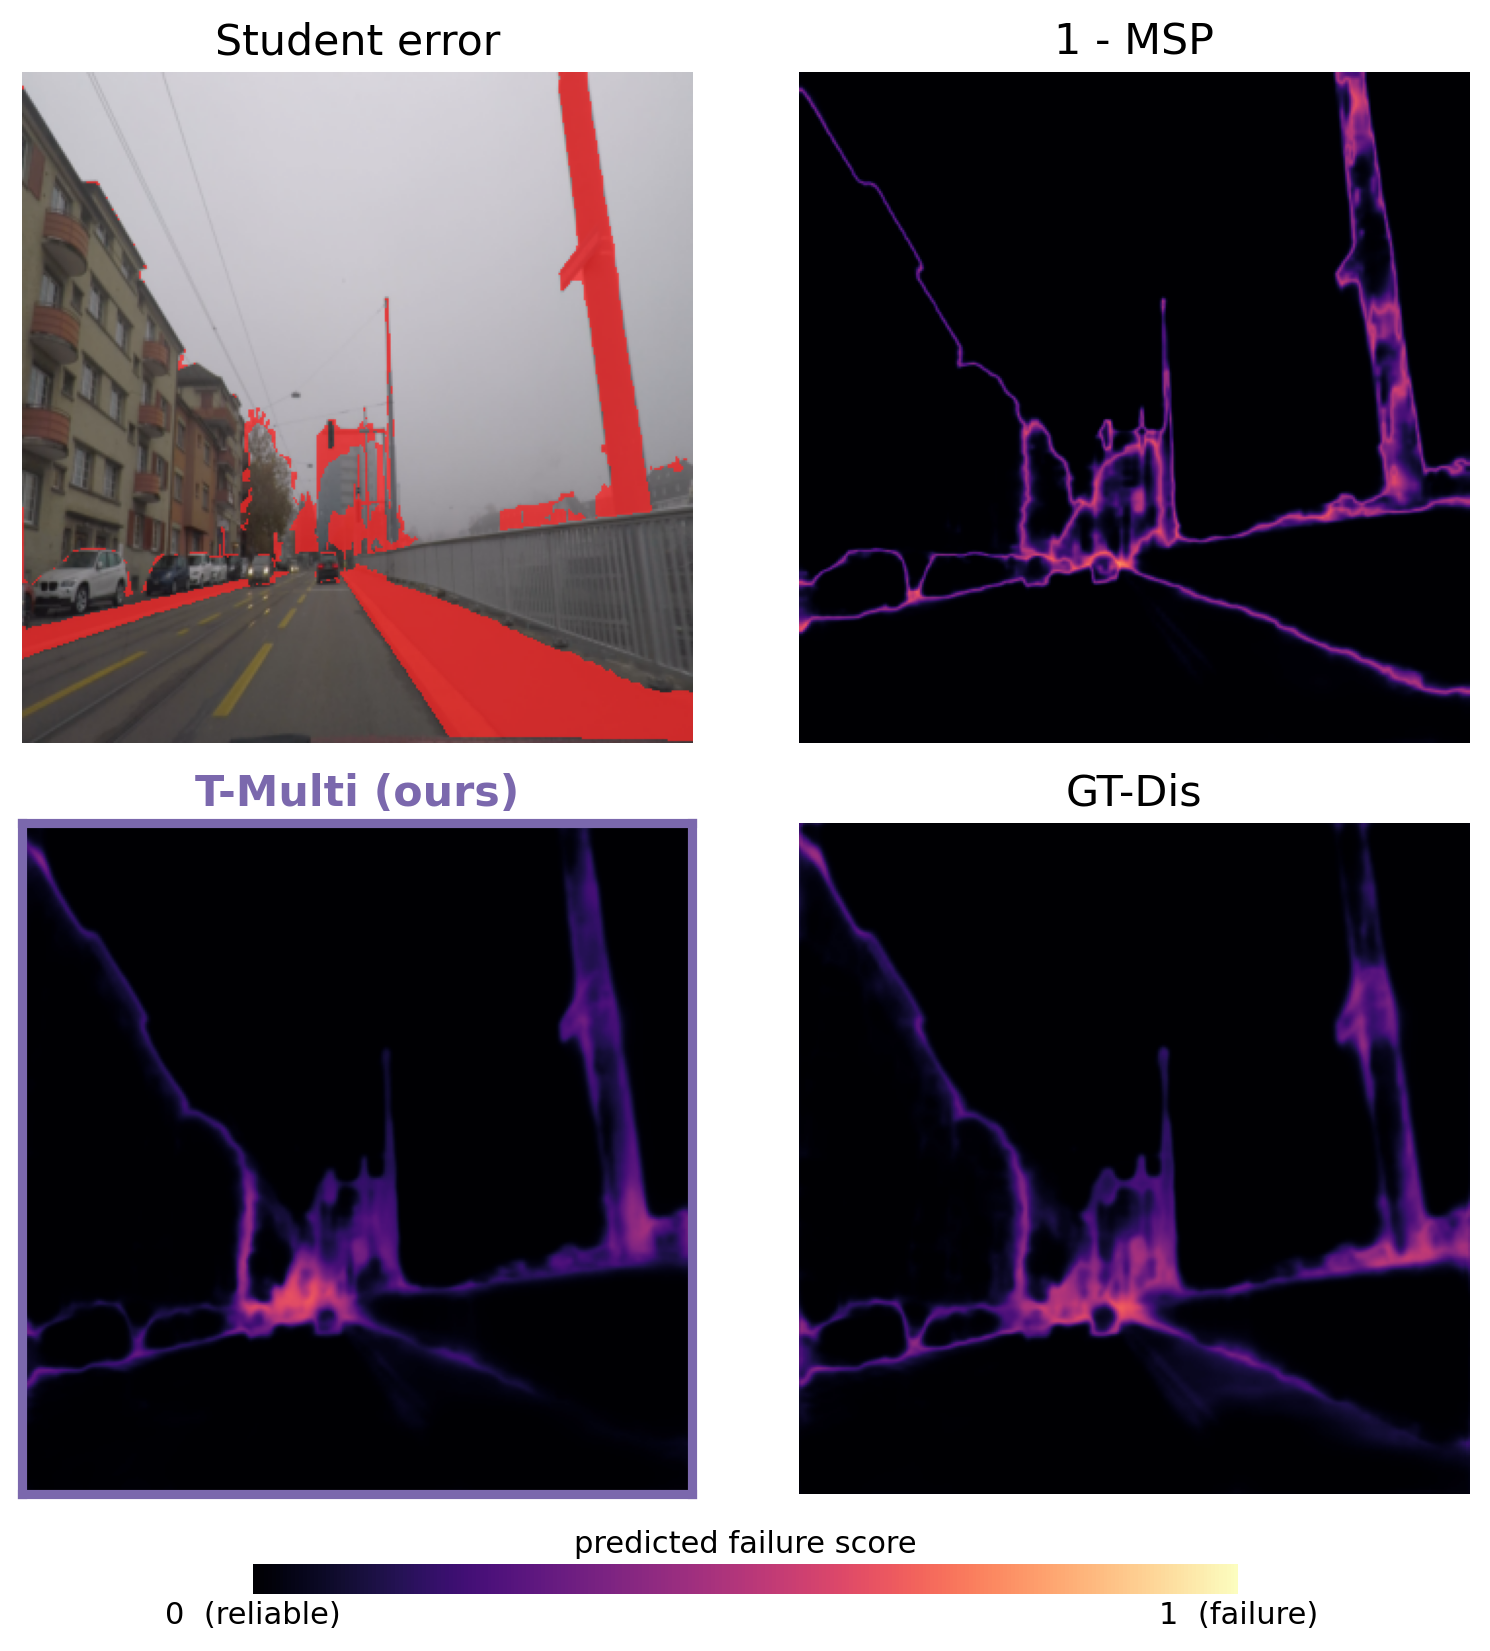
\includegraphics[width=1.0\linewidth]{fig_acdc_fog_strong.png}
  \caption{Qualitative failure detection on an ACDC fog example, shown across four out-of-distribution scenarios (mit-b1). The first panel shows student pixel error overlaid in red on the input image. The remaining panels show the predicted failure scores for $1{-}\mathrm{MSP}$, T-Multi (ours), and the GT-Dis baseline.$1{-}\mathrm{MSP}$ activates almost exclusively along object boundaries and misses the interior regions where the student fails. Both learned heads recover the boundary structure and additionally fire on failed interiors, where silent confident failures are most spatially concentrated.}


 \label{fig:snow-qual}
\end{figure}


\section{Selective prediction}


\begin{table}[H]
\centering
\small
\setlength{\tabcolsep}{4pt}
\caption{AURC (mit-b1). Images ranked by risk.}
\label{tab:augrc}
\begin{tabular}{lccccccc}
\toprule
 & MSP & MaxL & TempMSP & MC-D & GT-Dis & GT-Gap & \textbf{T-Multi} \\
\midrule
City & .422 & \win{.415} & .422 & .422 & .423 & .422 & .422 \\
ACDC & .634 & \win{.601} & .625 & .630 & .610 & .612 & .610 \\
IDD& .633 & .636 & .635 & \win{.632} & .634 & \win{.632} & \win{.632} \\
BDD& .533 & .529 & .531 & .529 & .521 & .524 & \win{.515} \\
\bottomrule
\end{tabular}
\end{table}


AURC is a threshold-free metric that measures the area under the risk-coverage curve. On BDD, T-Multi (0.515) beats MaxLogit (0.529) and GT-Dis (0.521). On ACDC, T-Multi ties GT-Dis (both 0.610). MaxLogit achieves the best AURC (0.601) on this dataset due to the condition-level separation in logit magnitudes. The learned heads offer no advantage over post-hoc methods for in-domain images.


\section{Risk-coverage curves}


\begin{figure}[H]
 \centering
 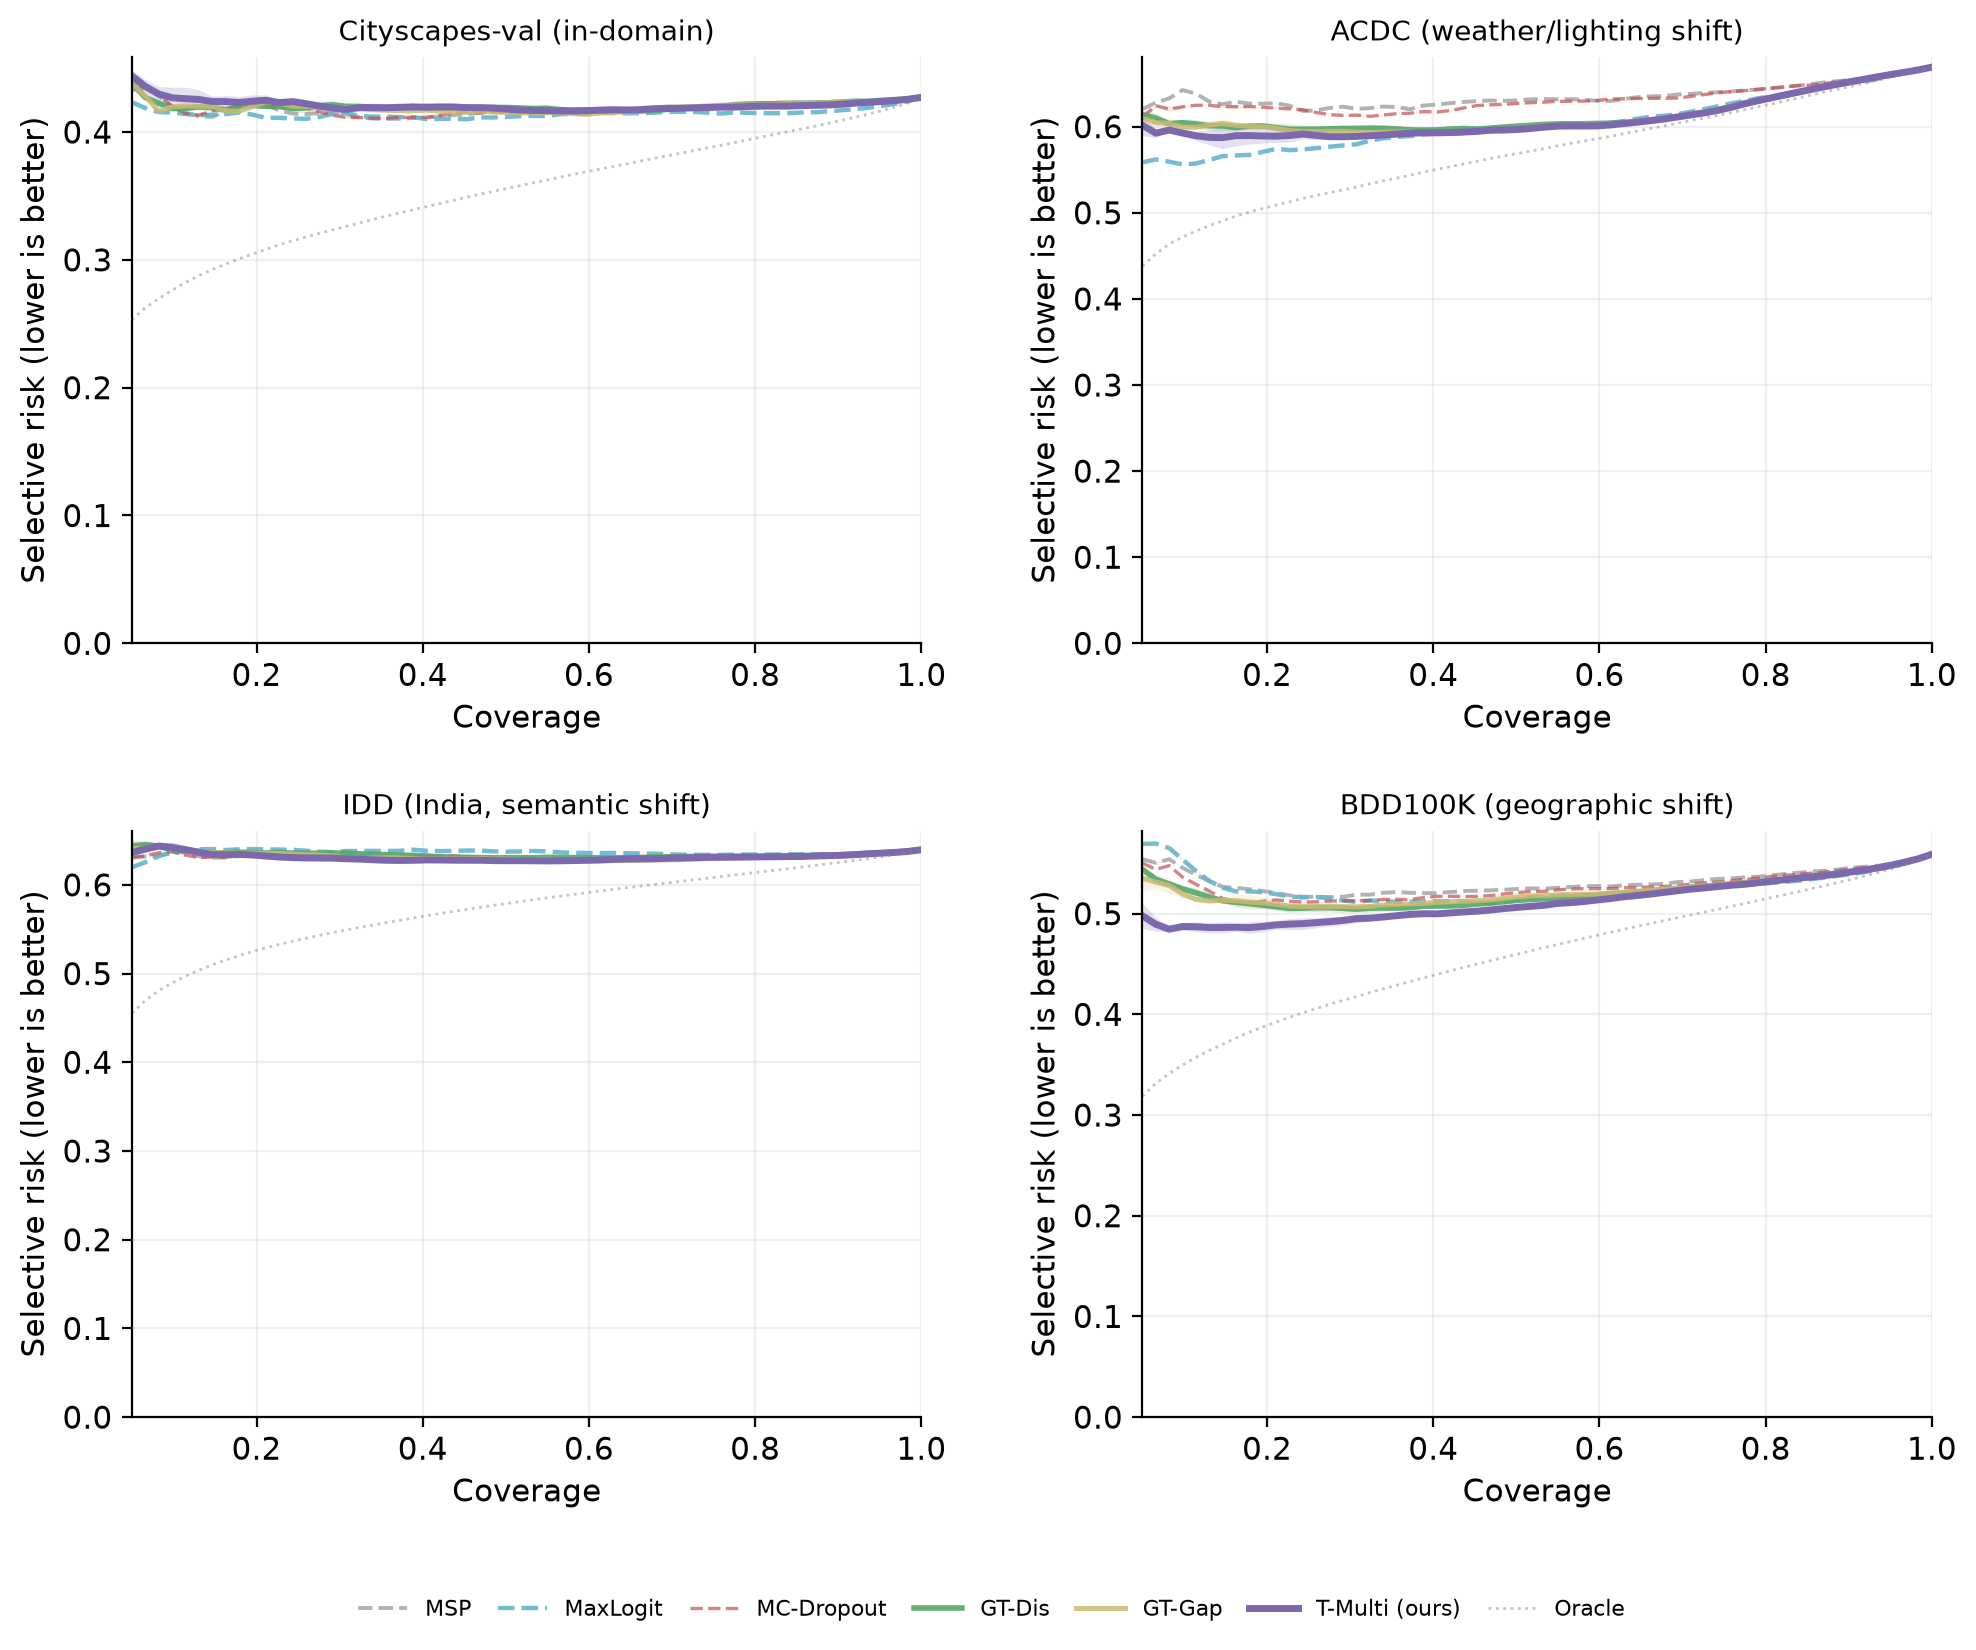
\includegraphics[width=0.9\linewidth]{fig_risk_coverage.png}
 \caption{Risk-coverage curves (mit-b1). T-Multi is competitive with GT baselines on ACDC and achieves the lowest selective risk on BDD.}
 \label{fig:rc}
\end{figure}


\section{Assets and licenses}
\label{app:assets-licenses}
We use existing datasets and pretrained models only under their original terms. Cityscapes is used for training and in-domain evaluation. ACDC is used for adverse-condition evaluation and is used under the official ACDC license for non-commercial use. IDD is used for geographic and semantic shift evaluation and is accessed through the official IDD portal. BDD100K is used for geographic and environmental shift evaluation under the official BDD100K terms. The SegFormer teacher and student architectures are based on the SegFormer model family, and the pretrained NVIDIA Hugging Face checkpoint used is licensed under the terms listed in the model card.


Released code is distributed under the repository license. Released checkpoints are provided for research use and remain subject to upstream model and dataset terms and do not include or redistribute raw dataset images or labels.


\newpage
\input{checklist.tex}


\end{document}